\chapter{Results}\label{chap:results_rankings}

Once the obtained rankings have been validated, it is possible to observe the resulting information. In this section, the main high-ranking drugs for the diseases under investigation will be discussed in detail. Before highlighting the results, however, it is necessary to state that all the results of an analysis such as the one performed by the project remain only an intuition that is meant to represent a direction for actual biological studies on the experimental evidence obtained from this first approach.
~\\[0.3cm]
The vast majority of drugs detected in the high rankings turn out to be \textbf{anti-cancer treatments}, examples being ``Entinostat", ``Vorinostat" and ``Belinostat", detected in the ranking for ``Propionic Acidemia"~\cite{drugbank}.

Also of interest are the findings of treatments for ``\textbf{Alzheimer}"'s and ``\textbf{Parkinson}"'s, found in the ``Methylmalonic Acidemia" and ``Propionic Acidemia" rankings, respectively, represented by the drugs ``Gantenerumab" and ``Amantadine"~\cite{drugbank}.

Another case is that of ``Rabies Immune Globuline", a solution of antibodies used to prevent ``\textbf{Rabies}" after an exposure, found to be both a good candidate in the ranking of ``Homocystinuria" and ``Propionic Acidemia"~\cite{drugbank}.
~\\[0.01cm]
Other findings are also confirmed or at least supported by certain correlations, interactions and symptoms already found in the scientific literature when referring to the diseases in analysis.
For example, ``Vitamin B12" and ``Hydroxocobalamin" were found in the highest positions for ``Methylmalonic Acidemia", a disease that appears to be related ~\cite{pubmed1} to the deficiency of precisely ``Vitamin B12", of which ``Hydroxocobalamin" is a synthetic substitute~\cite{drugbank}.
Similarly, correlations have been found between drugs that seems related to ``Hypercalcemia", such as ``Zoledronic Acid" and ``Pamidronic Acid", and the ranking of ``Hyperglycinemia", a metabolic disease that seems to have correlations~\cite{pubmed2} with the former~\cite{drugbank}.
~\\[0.3cm]
Finally, an honourable mention goes to ``Foreskin Keratinocyte (Neonatal)", a drug that ranks highly for the vast majority of diseases analysed ~\cite{drugbank}.

\begin{figure}[h!]
    \centering
    \begin{subfigure}[b]{0.3\textwidth}
         \centering
          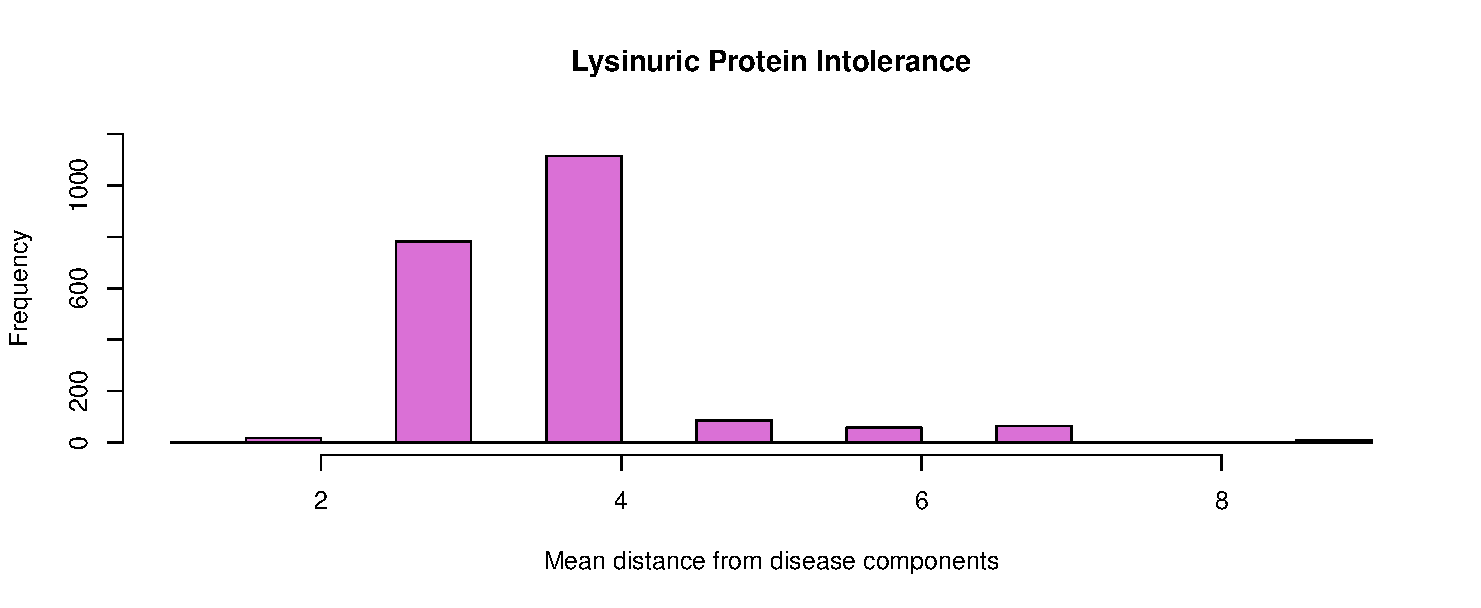
\includegraphics[scale=0.25]{Images/Lisinuric Protein Intolerance.pdf}
         \caption{LPI}
         \label{fig:Lisinuric}
     \end{subfigure}
     \hfill
     \begin{subfigure}[b]{0.3\textwidth}
         \centering
         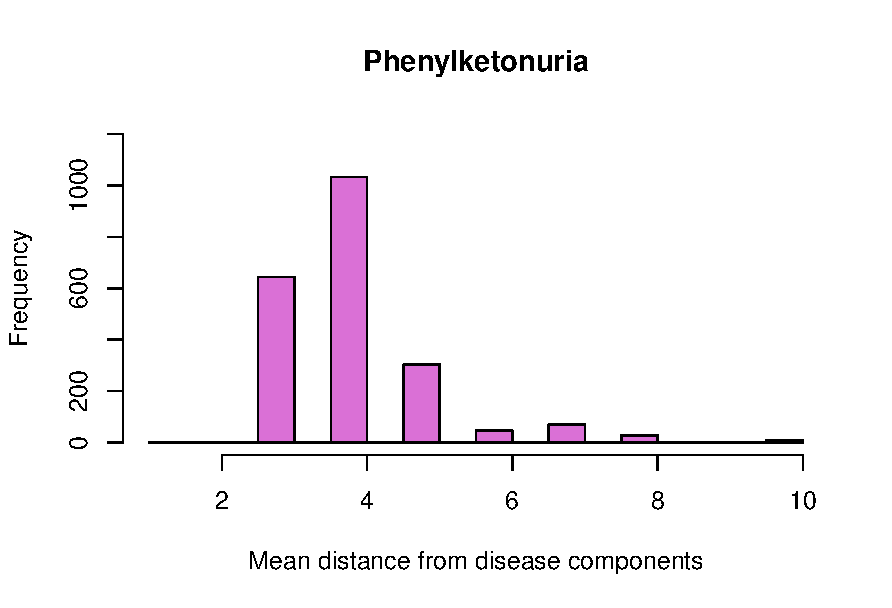
\includegraphics[scale=0.25]{Images/Phenylketonuria.pdf}
         \caption{Phenylketonuria}
         \label{fig:Phenylketonuria}
     \end{subfigure}
     \hfill
     \begin{subfigure}[b]{0.3\textwidth}
         \centering
         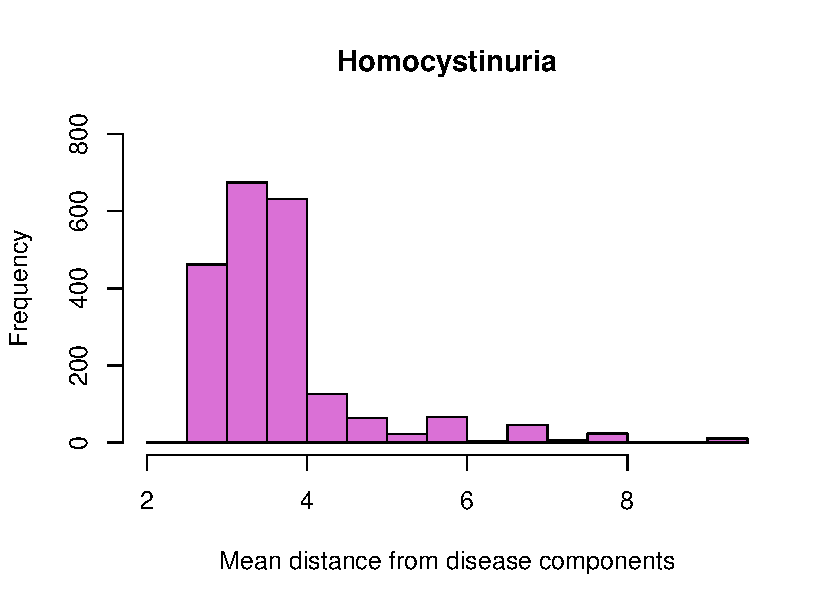
\includegraphics[scale=0.25]{Images/Homocystinuria.pdf}
         \caption{Homocystinuria}
         \label{fig:Homocystinuria}
     \end{subfigure}
     \hfill
     \begin{subfigure}[b]{0.3\textwidth}
         \centering
         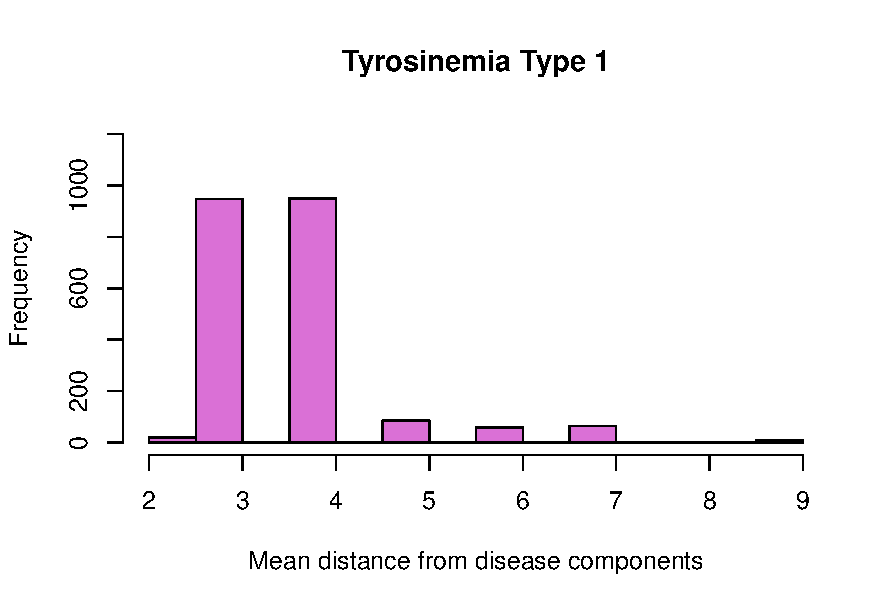
\includegraphics[scale=0.25]{Images/Tyrosinemia Type I.pdf}
         \caption{Tyrosinemia Type I}
         \label{fig:Tyrosinemia Type I}
     \end{subfigure}
     \hfill
     \begin{subfigure}[b]{0.3\textwidth}
         \centering
         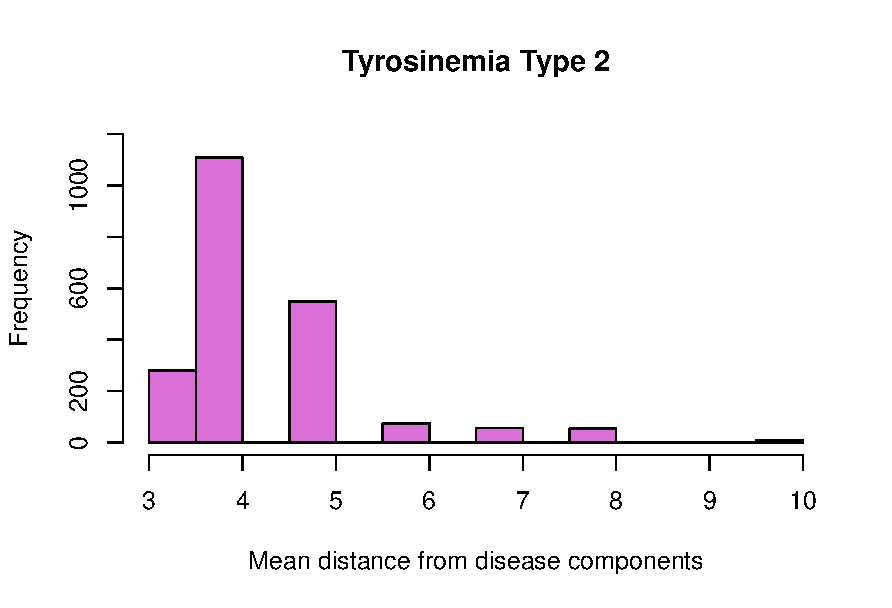
\includegraphics[scale=0.25]{Images/Tyrosinemia Type II.pdf}
         \caption{Tyrosinemia Type II}
         \label{fig:Tyrosinemia Type II}
     \end{subfigure}
     \hfill
     \begin{subfigure}[b]{0.3\textwidth}
         \centering
         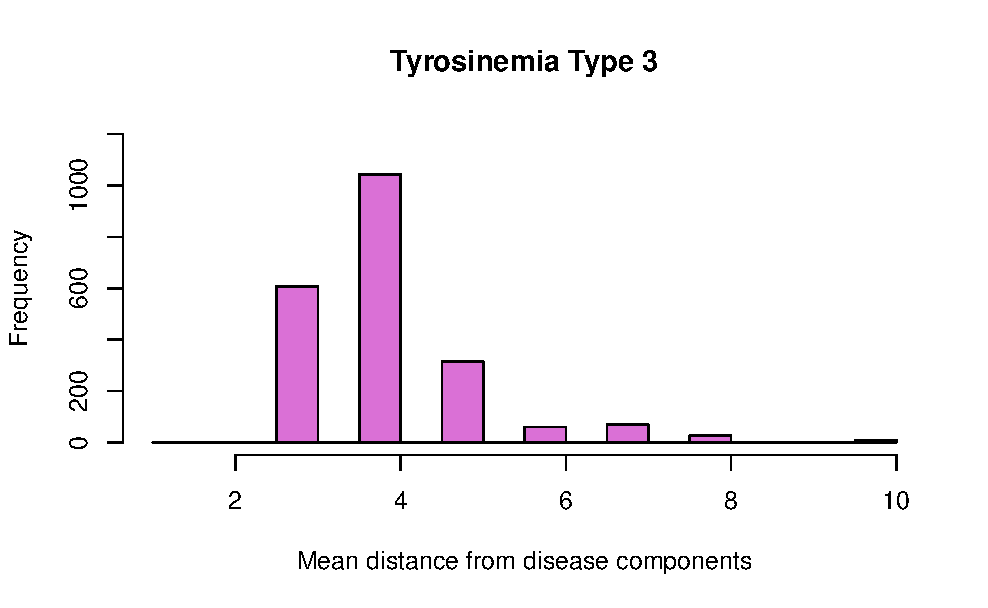
\includegraphics[scale=0.25]{Images/Tyrosinemia Type III.pdf}
         \caption{Tyrosinemia Type III}
         \label{fig:Tyrosinemia Type III}
     \end{subfigure}
     \hfill
     \begin{subfigure}[b]{0.3\textwidth}
         \centering
         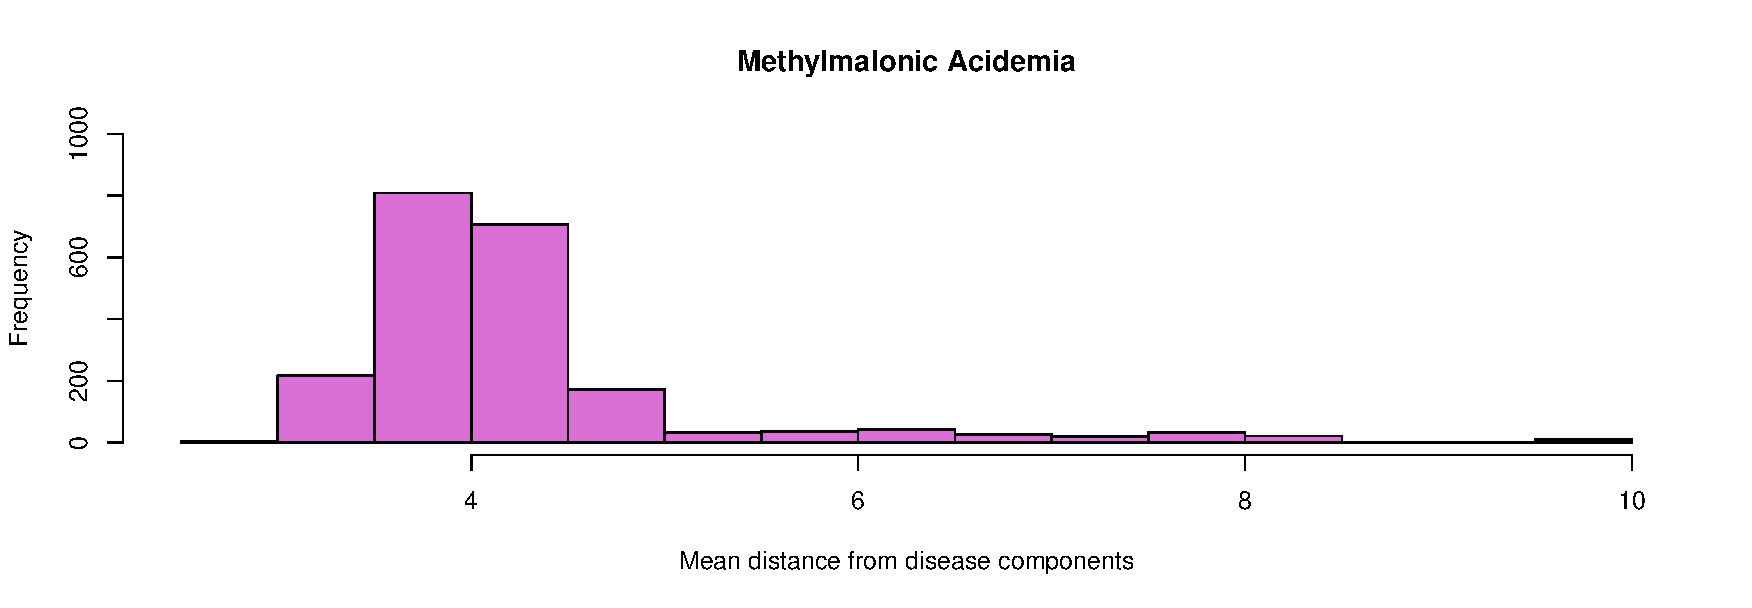
\includegraphics[scale=0.25]{Images/Methylmalonic Acidemia.pdf}
         \caption{Methylmalonic A.}
         \label{fig:Methylmalonic Acidemia}
     \end{subfigure}
     \hfill
     \begin{subfigure}[b]{0.3\textwidth}
         \centering
         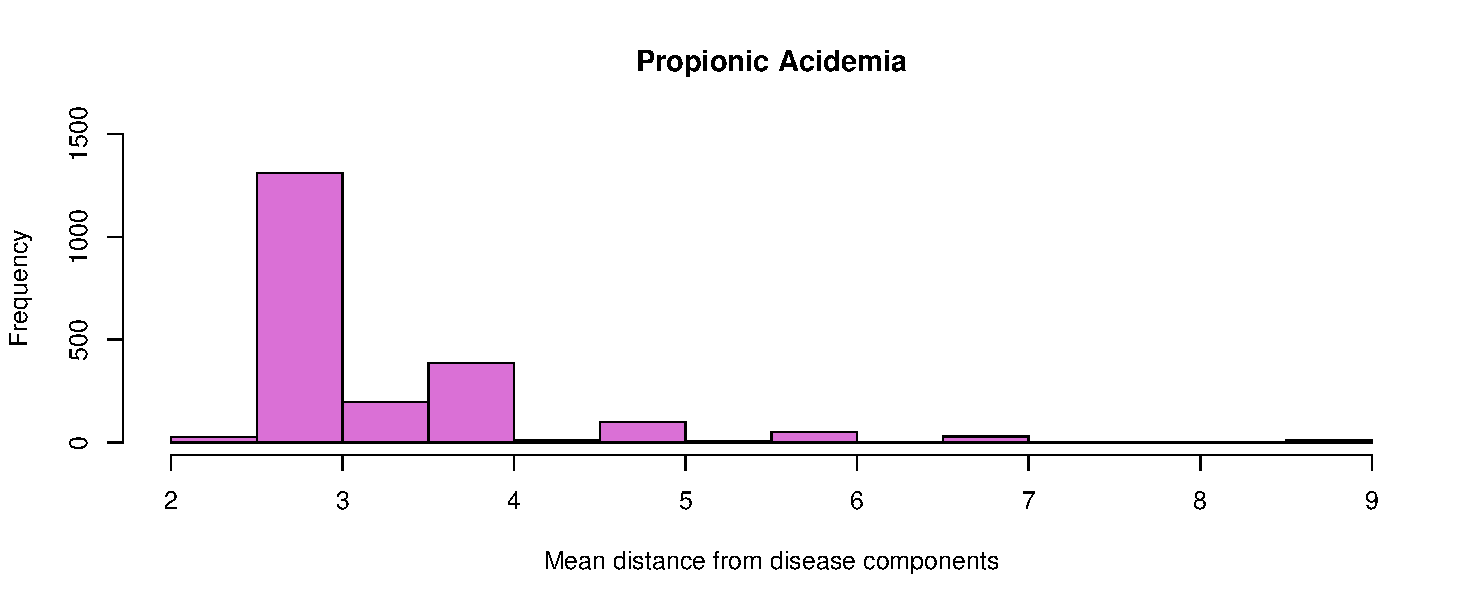
\includegraphics[scale=0.25]{Images/Propionic Acidemia.pdf}
         \caption{Propionic Acidemia}
         \label{fig:Propionic Acidemia}
     \end{subfigure}
     \hfill
     \begin{subfigure}[b]{0.3\textwidth}
         \centering
         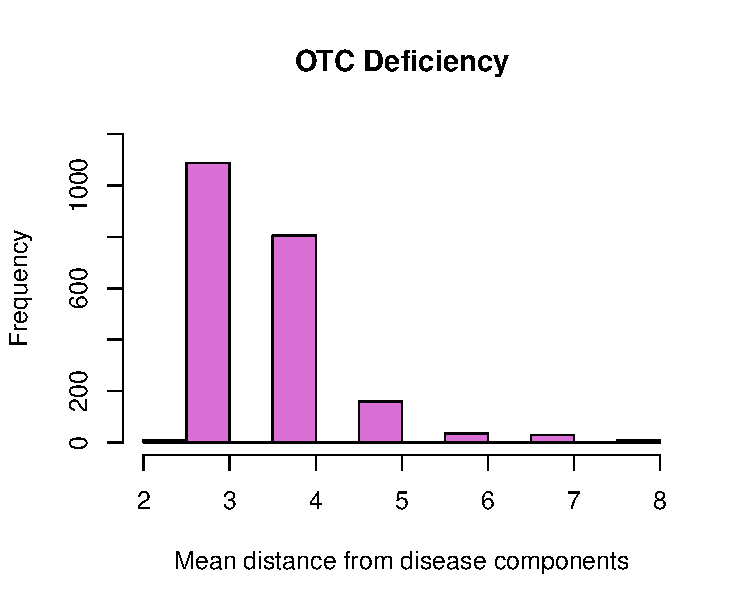
\includegraphics[scale=0.25]{Images/OTC Deficiency.pdf}
         \caption{OTC Deficiency}
         \label{fig:OTC}
     \end{subfigure}
     \hfill
      \begin{subfigure}[b]{0.3\textwidth}
         \centering
         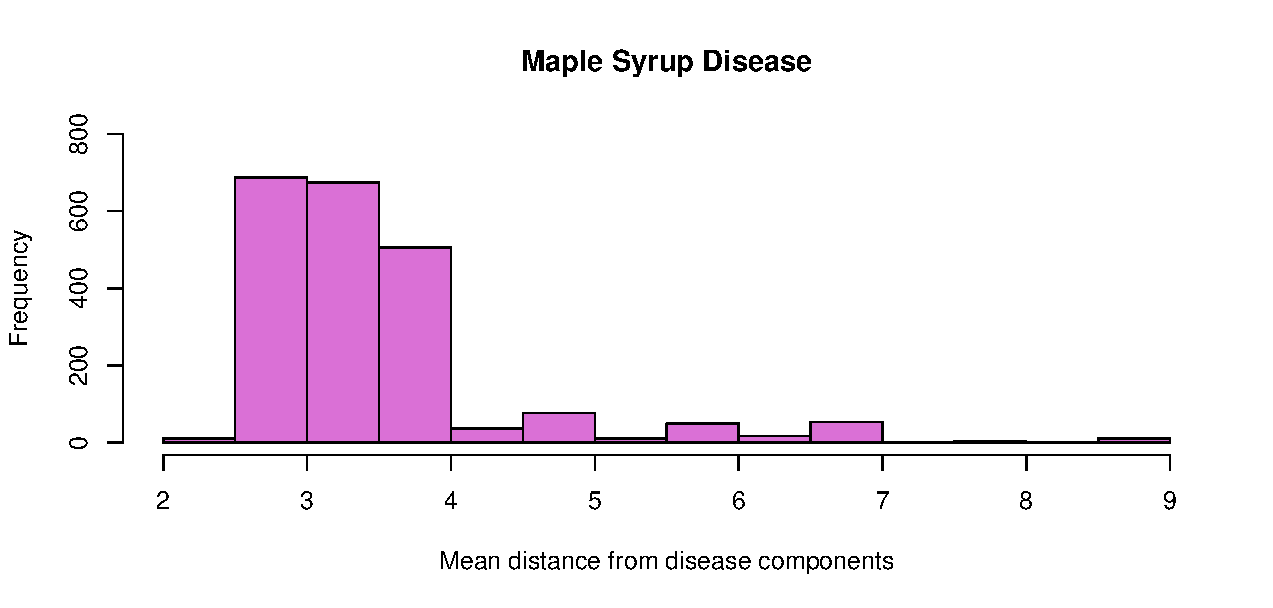
\includegraphics[scale=0.25]{Images/Maple Syrup Disease.pdf}
         \caption{Maple Syrup Disease}
         \label{fig:Maple Syrup}
     \end{subfigure}
     \hfill
     \begin{subfigure}[b]{0.3\textwidth}
         \centering
         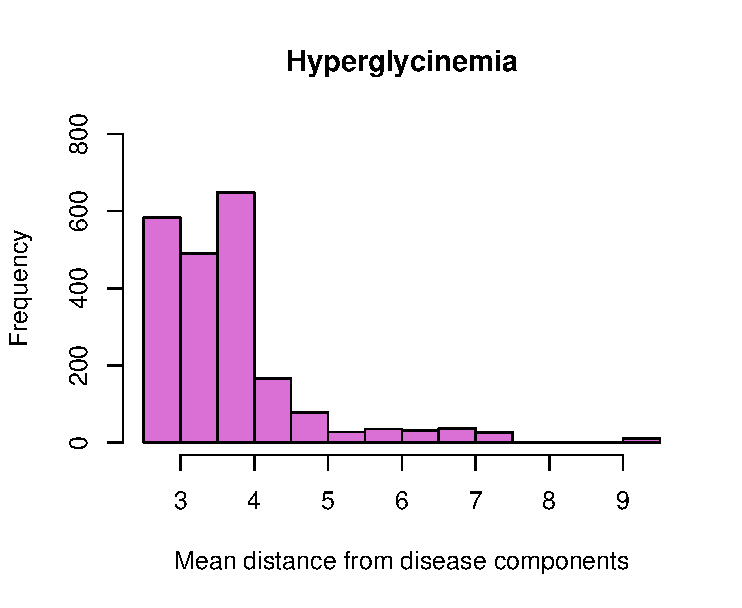
\includegraphics[scale=0.25]{Images/Hyperglycinemia.pdf}
         \caption{Hyperglycinemia}
         \label{fig:Hyperglycinemia}
     \end{subfigure}
     \hfill
     \begin{subfigure}[b]{0.3\textwidth}
         \centering
         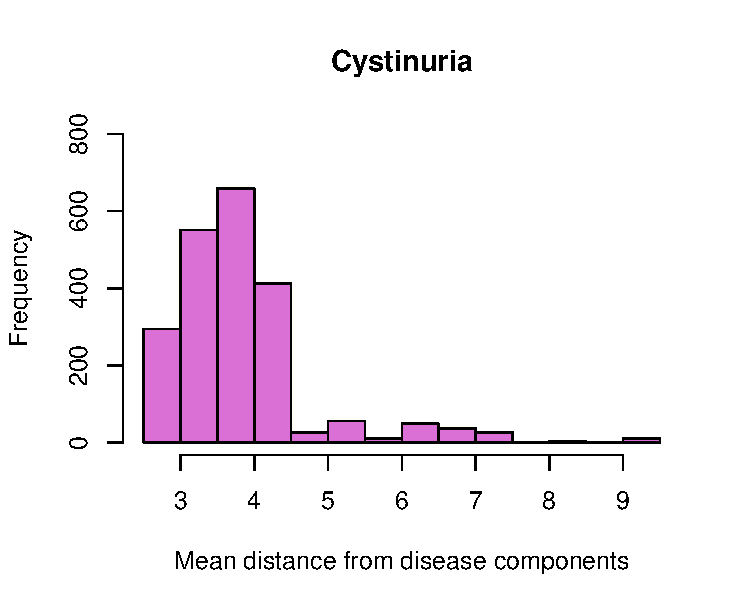
\includegraphics[scale=0.25]{Images/Cystinuria.pdf}
         \caption{Cystinuria}
         \label{fig:Cystinuria}
     \end{subfigure}
     \hfill
    \caption{Drugs mean distances frequency distribution for each disease's ranking}
    \label{fig:results}
\end{figure}
\FloatBarrier